% Tento soubor nahraďte vlastním souborem s přílohami (nadpisy níže jsou pouze pro příklad)
% This file should be replaced with your file with an appendices (headings below are examples only)

% Umístění obsahu paměťového média do příloh je vhodné konzultovat s vedoucím
% Placing of table of contents of the memory media here should be consulted with a supervisor
%\chapter{Obsah přiloženého paměťového média}

%\chapter{Manuál}

%\chapter{Konfigurační soubor} % Configuration file

%\chapter{RelaxNG Schéma konfiguračního souboru} % Scheme of RelaxNG configuration file

%\chapter{Plakát} % poster

\chapter{Complete oVirt virtual machine dialog dependency graph} \label{graph}
\newpage
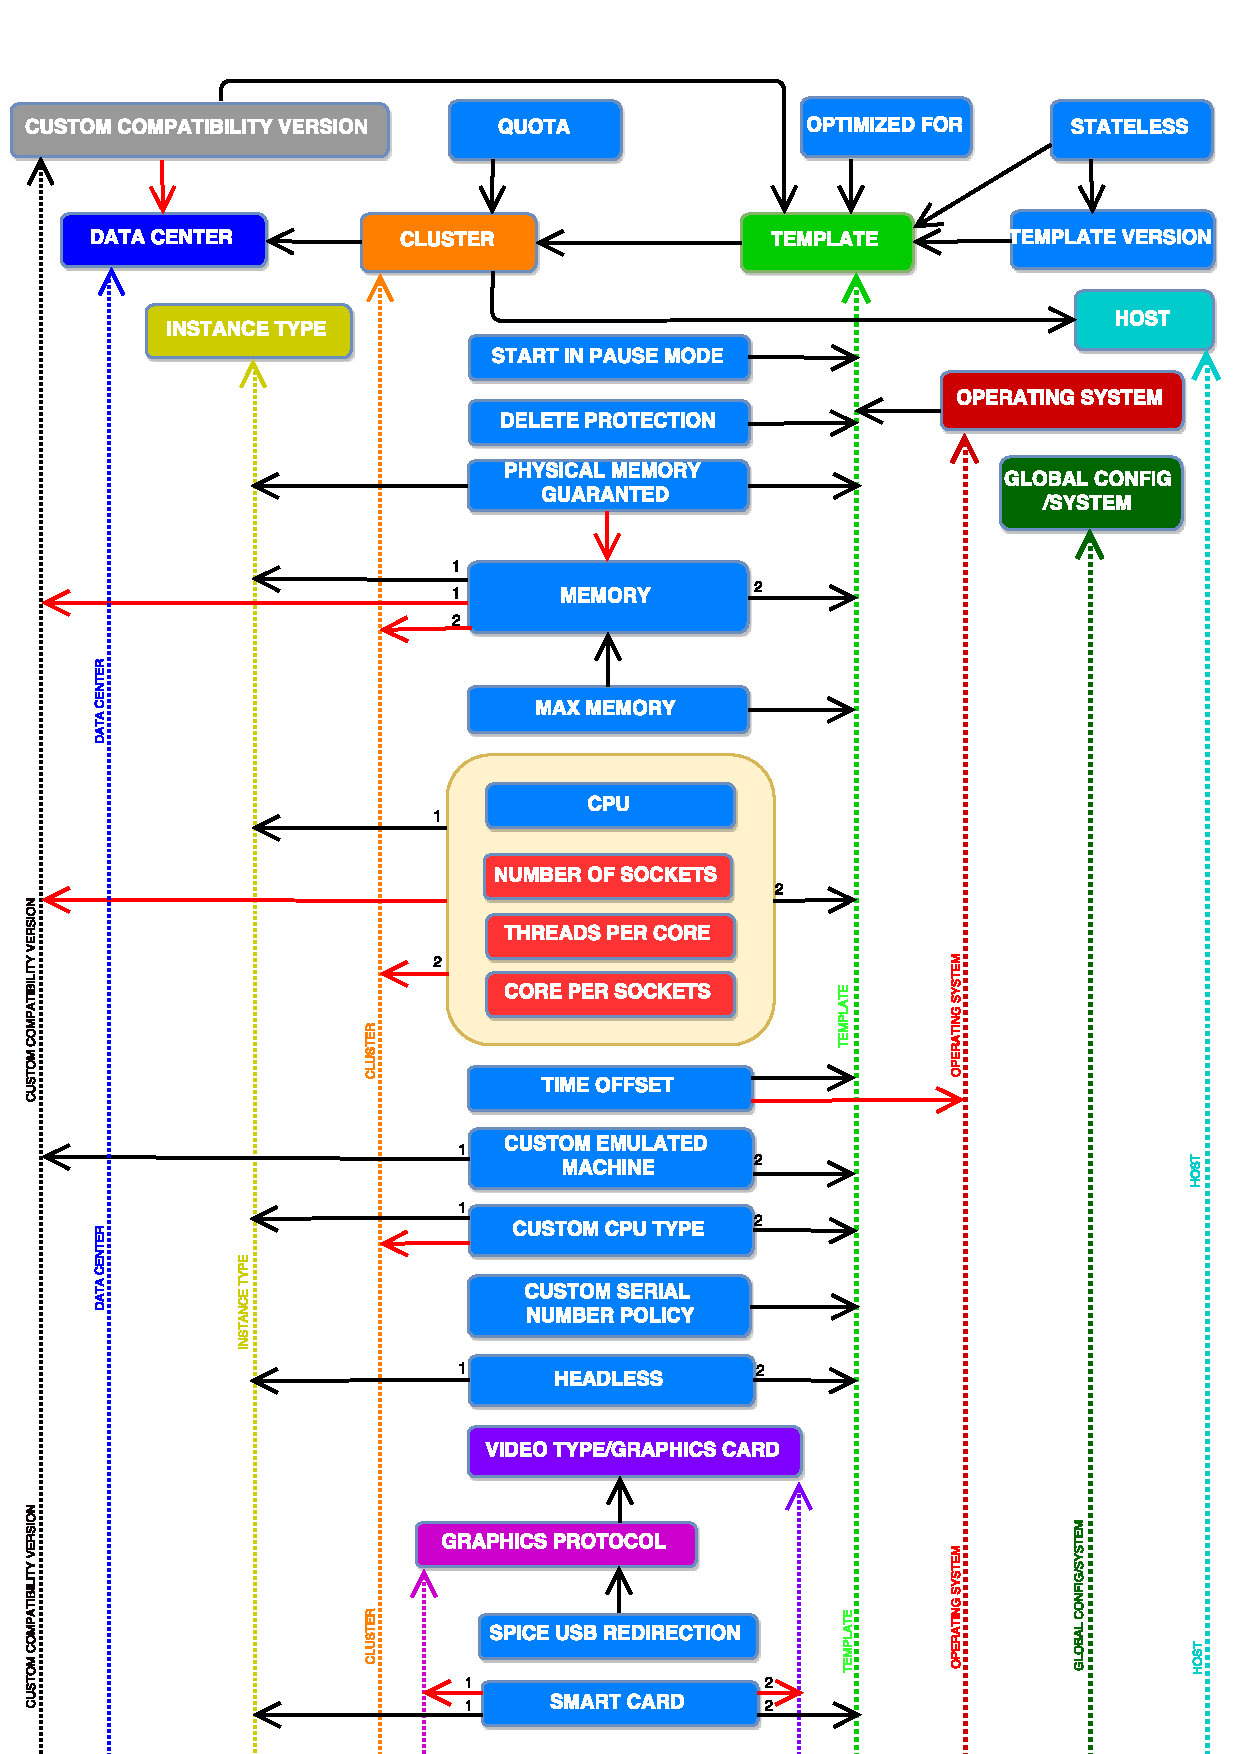
\includegraphics[page=1, width=1.05\textwidth, angle=0]{DependencyGraph}
\newpage
\includegraphics[page=2, width=1.05\textwidth, angle=0]{DependencyGraph}
\newpage
\includegraphics[page=3, width=1.05\textwidth, angle=0]{DependencyGraph}

\chapter{Installation guide} \label{install}

\section{Prerequisites}
Note: Work done by this thesis have partially been included in oVirt 4.1 release. To run the application in the most present version, it is recommended to use the development mode with engine url. 

\begin{enumerate}
\item An oVirt engine running with configured hosts, disks and networks.  
\item A ManageIQ instance running and configured to manage the oVirt engine (ManageIQ variant - read only mode)
\end{enumerate} 

\section{oVirt API variant installation - Fedora/Red Hat Enterprise Linux}
\begin{enumerate}

\item Copy the contents of attached CD 
\item Open terminal
\item Navigate to directory of copied content
\item Make sure that you are in correct folder (oVirt API) \texttt{cd ovirt-web-ui}
\item Make sure npm is installed \texttt{yum install npm}
\item Install yarn \texttt{npm install yarn}
\item Install all project dependencies by running \texttt{yarn install}
\item Run oVirt-web-ui \texttt{ENGINE\char`_URL=https://engine\char`_address yarn start} (change the url to your oVirt engine)
\item Firefox window should automatically open with application, if not application url should be displayed in output of terminal window)

\end{enumerate} 
\section{ManageIQ API variant installation - Fedora/Red Hat Enterprise Linux}
\begin{enumerate}

\item Copy the contents of attached CD 
\item Open terminal
\item Navigate to directory of copied content
\item Make sure that you are in correct folder (ManageIQ API) \texttt{cd manageiq}
\item Make sure npm is installed \texttt{yum install npm}
\item Install yarn \texttt{npm install yarn}
\item Install and update all required project dependencies by running \texttt{yarn install}
\item Run oVirt-web-ui \texttt{ENGINE\char`_URL=https://engine\char`_address yarn start} (change the url to your oVirt engine)
\item Firefox window should automatically open with application, if not application url should be displayed in output of terminal window)

\end{enumerate} 
